%% LyX 2.0.0 created this file.  For more info, see http://www.lyx.org/.
%% Do not edit unless you really know what you are doing.
\documentclass[english]{article}
\usepackage[T1]{fontenc}
\usepackage[utf8]{luainputenc}
\usepackage{amsmath}
\usepackage{amssymb}
\usepackage{graphicx}
\usepackage{babel}
\begin{document}

\title{Final Exam}


\author{Shuowen Wei}

\maketitle

\part{Theoretical }
\begin{description}
\item [{Problem}] 24.1 
\end{description}
Proof:

(c).

True:

Since the eigenvalues are the roots of the characteristic polynomial
of $A$, i.e $P(\lambda)=det(\lambda I-A)=0$, $A$ is real matrix
so all the parameters in are real, and the complex roots always appear
in pairs. If $\lambda$ is the root of $P(\lambda)=0$, so is $\bar{\lambda}$,
then $\bar{\lambda}$ is also the eigenvalue of $A$.

(f).

True:

This is the\textbf{ }statement of \textbf{Theorem 5.5}, we just repeat
the proof on Sept. 8's note here: if $A$ is hermitian matrix, then
$A$ has a complete set of orthogonal eigenvectors and all of the
eigenvectors are real. Then $A$ has eigenvalue decomposition as $A=Q\Lambda Q^{*}=Q|\Lambda|sign(\Lambda)Q^{*}$,
where the entries in the diagonal of $\Lambda$ are the eigenvalues
of $A$ and $Q$ is unitary matrix. Just denote $Q$ as $U$ and $sign(\Lambda)Q^{*}$
as $V^{*}$, then we have $\Sigma=|\Lambda|$, as desired. 
\begin{description}
\item [{Problem}] 24.4
\end{description}
Proof:

(a).

$(\Longrightarrow)$

Suppose $\lambda$ is $A$'s arbitrary eigenvalue and $x$ is its
corresponding eigenvector, then $Ax=\lambda x$, hence $\lambda^{2}x=\lambda Ax=A\lambda x=AAx=A^{2}x$,
repeat this way we can get that $\lambda^{n}x=A^{n}x$. By using the
same idea we did in Exercise 3.2 (we already proved that on \textbf{Project
1}), $|\lambda|^{n}\,||x||=||\lambda^{n}x||=||A^{n}x||\leq||A^{n}||\,||x||$,
thus we have $|\lambda^{n}|\leq||A^{n}||$.

So if $lim_{n\rightarrow\infty}|\lambda^{n}|\leq lim_{n\rightarrow\infty}||A^{n}||=0$,
then $lim_{n\rightarrow\infty}|\lambda^{n}|=0$, then $|\lambda|<1$,
since $\lambda$ is arbitrary, then $\rho(A)<1$.

$(\Longleftarrow)$

Since $A\in\mathbb{C}^{m\times m}$ is a square matrix, by \textbf{Theorem
24.9} that $A$ has a Schur factorization $A=QTQ^{*}$ where $Q$
is unitary and $T$ is upper-triangular. Note that $A$ and $T$ are
similar then they have the same eigenvalues, since $T$ is upper-triangular,
then eigenvalues of $A$ necessarily appear on the diagonal of $T$.
Now we have

\[
A^{n}=(QTQ^{*})^{n}=QT^{n}Q^{*}
\]


If $\rho(A)=\rho(T)<1$, then every entries in $T$'s diagonal is
less than 1. Since $T$ is upper triangular, then $lim_{n\rightarrow\infty}T^{n}=O$,
which implies that $lim_{n\rightarrow\infty}||A^{n}||=lim_{n\rightarrow\infty}||Q||\,||T^{n}||\,||Q^{*}||=0$.

(b). 

The spectral abscissa of a matrix $A$ denoted as $\alpha(A)=max\, Re(\lambda)$
where $\lambda$ is the eigenvalue of $A$.

The definition of $e^{tA}$ is $e^{tA}=\sum_{k=0}^{\infty}\frac{1}{k!}(tA)^{k}$,
and it has several properties as follows:

1. $e^{t(TAT^{-1})}=Te^{tA}T^{-1}$ 

2. $e^{t(A+B)}=e^{tA}e^{tB}$ for all $B$ with $AB=BA$

3. $A=diag(A_{1},\, A_{2},...A_{m})\Longrightarrow e^{tA}=diag(e^{tA_{1}},e^{tA_{2}},...,e^{tA_{m}})$

Since $A\in\mathbb{C}^{m\times m}$ is a square matrix, by \textbf{Theorem
24.9} that $A$ has a Schur factorization $A=QTQ^{*}$ where $Q$
is unitary and $T$ is upper-triangular. Then $e^{tA}=Qe^{tT}Q^{*}$.
Since $T$'s diagonal entries are $A$'s eigenvalues, denote $T$
as $T=\lambda I+N$ where $N$ is the rest of the entries in $T$
except the eigenvalues, it's a kind like {}``deficient upper triangular
matrix''. For any eigenvalue $\lambda$ that might be complex, $\lambda=Re(\lambda)+iIm(\lambda)$,
where $Re(\lambda)$ and $Im(\lambda)$ are real, then $|e^{\lambda}|=|e^{Re(\lambda)}|\,|e^{iIm(\lambda)}|=|e^{Re(\lambda)}|.$

Then we have $e^{tT}=e^{t\lambda}e^{tN}=e^{t\lambda}(1+tN+\cdots+\frac{1}{(m-1)!}(tN)^{m-1})$,
thus

\[
||e^{tA}||=||Qe^{tT}Q^{*}||=|e^{t\lambda}|\,||e^{tN}||=|e^{tRe(\lambda)}|(1+t||N||+\cdots+\frac{1}{(m-1)!}t{}^{m-1}||N||^{m-1})
\]


Then $\forall\lambda,\,\exists M>0$, such that $||e^{tA}||=Me^{tRe(\lambda)}\leq Me^{t\alpha(A)}$, 

Since $\lambda$ is arbitrary eigenvalue of $A$, thus $lim_{t\rightarrow\infty}||e^{tA}||=0\Longleftrightarrow\alpha(A)<0$.
\begin{description}
\item [{Problem}] 25.1(a)
\end{description}
Proof:

Since $A$ is tridiagonal and hermitian, then $A$ is full rank. For
any $\lambda\in\mathbb{C}$, we have

\[
A-\lambda I=\left[\begin{array}{ccccc}
a_{11}-\lambda & a_{12} & 0 & \cdots & 0\\
a_{12} & a_{22}-\lambda & a_{23} & \cdots & 0\\
0 & a_{23} & a_{3}-\lambda & \cdots & 0\\
\vdots & \vdots & \vdots & \ddots & a_{m-1,m}\\
0 & 0 & 0 & a_{m-1,m} & a_{mm}-\lambda
\end{array}\right]
\]


since the subdiagonal and superdiagonal entries $a_{12},\, a_{23},\,...a_{m-1,m}$
are nonzeros, then after row operation we can still get at least $m-1$
rows of the matrix with first entry of each row is nonzero, thus $A-\lambda I$
has at least rank $m-1$.

Since $A$ is hermitian, by \textbf{Theorem 24.7}, $A$ is unitarily
diagonalizable, then we have that $A=Q\Lambda Q^{*}$, where $Q$
is unitary matrix and $\Lambda$ is diagonal matrix with enreies are
the eigenvalues of $A$ , let $\Lambda=diag(\lambda_{1},\,\lambda_{2},\,...,\,\lambda_{m})$,
so

\[
A-\lambda I=Q\Lambda Q^{*}-Q\lambda IQ^{*}=Q\left[\begin{array}{cccc}
\lambda_{1}-\lambda & 0 & \cdots & 0\\
0 & \lambda_{2}-\lambda & \cdots & 0\\
\vdots & \vdots & \ddots & \vdots\\
0 & 0 & \cdots & \lambda_{m}-\lambda
\end{array}\right]Q^{*}
\]


Since $\lambda$ is arbitrary in $\mathbb{C}$, so if $A$ has any
two same eigenvalues, say $\lambda_{i},\,\lambda_{j}$, then let $\lambda=\lambda_{i}$,
then $Q(\Lambda-\lambda I)Q^{*}$ will has rank at most $m-2$, which
contradicts that it has at least rank $m-1,$ so every eigenvalues
of $A$ are distinct. 
\begin{description}
\item [{Problem}] 4
\end{description}
Solution: 

For any matrix $A\in C^{m\times n}$, $m>n$, the condition number
in terms of the singular value of $A$ is 

\[
k(A)=\parallel A\parallel\parallel A^{\dagger}\parallel=\frac{\sigma_{1}}{\sigma_{n}}
\]


where $\sigma_{1}$is largest singular value of $A$ and $\sigma_{n}$
is the smallest singular value of $A$. If $A$ is not full rank,
then $\sigma_{n}=0$, thus $k(A)=\infty$.
\begin{description}
\item [{Problem}] 5
\end{description}
Proof:

I think something is wrong with this question. Why the conjugancy
of $A$ by two vectors is still a matrix? And what's the subspace
of a vector space? 
\begin{description}
\item [{Problem}] 6
\end{description}
Proof:

Suppose the matrix $A$'s rank is $r\,(\leq min(m,n))$, then by \textbf{Theorem
5.9}, that for any $k$ with $0\leq k\leq r$, we have the best rank-k
approximation of $A$ is

\[
||A-A_{k}||_{F}=\underset{B\in\mathbb{C}^{m\times n}}{inf}||A-B||_{F}=\sqrt{\sigma_{k+1}+\sigma_{k+2}+\cdots+\text{\ensuremath{\sigma}}_{r}}\,\,\,\,\,\,\,(*)
\]


Since $A$ has SVD decomposition $A=\sum_{i=1}^{n}\sigma_{i}u_{i}v_{i}^{*}$
and for $1\leq k\leq r$ we have $A_{k}=\sum_{i=1}^{k}\sigma_{i}u_{i}v_{i}^{*}$,
and each $\sigma_{i}u_{i}v_{i}^{*}$ is a rank one matrix. The SVD
of $A$ is unique if the sign of $U$ or $V$ is fixed, since for
any $k$, $\sigma_{k}\geq\sigma_{k+1}$. If $\sigma_{k}=\sigma_{k+1}$,
then we will get two matrix $A_{1}$ and $A_{2}$ just with the last
column different, one is $\sigma_{k}u_{k}v_{k}^{*},$the other one
is $\sigma_{k+1}u_{k+1}v_{k+1}^{*}$ such that, by formula ({*}) 

\[
||A-A_{k}||_{F}=\sqrt{\sigma_{k+1}+\sigma_{k+2}+\cdots+\text{\ensuremath{\sigma}}_{r}}=\sqrt{\sigma_{k}+\sigma_{k+2}+\cdots+\text{\ensuremath{\sigma}}_{r}}=||A-A_{k+1}||_{F}
\]


Hence the besk rank-k approximation is not unique. So $A_{k}$ is
the unique solution to formula ({*}) to minimise the problem if and
only if $\sigma_{k}>\sigma_{k+1}$.
\begin{description}
\item [{Problem}] 7
\end{description}
Proof:

By the definition of F-norm, $||A||_{F}^{2}=tr(A^{*}A)$, then first
of all, we will prove that for any matrix $B$ and $C$, $||AB+(I-AA^{\dagger})C||_{F}^{2}=||AB||_{F}^{2}+||(I-AA^{\dagger})C||_{F}^{2}$
holds.

\[
||AB+(I-AA^{\dagger})C||_{F}^{2}
\]


\[
=(AB+(I-AA^{\dagger})C))^{*}(AB+(I-AA^{\dagger})C))
\]


\[
=(AB)^{*}(AB)+((I-AA^{\dagger})C)*((I-AA^{\dagger})C)+(AB)^{*}(I-AA^{\dagger})C+((I-AA^{\dagger})C)^{*}(AB)
\]


Since Moore-Penrose peseudoinverse $A^{\dagger}$ has properties $A^{*}AA^{\dagger}=A^{*}$
and $A^{\dagger*}A^{*}A=A$, then

\[
(AB)^{*}(I-AA^{\dagger})C=O\, and\,((I-AA^{\dagger})C)^{*}(AB)=O
\]


thus

\[
||AB+(I-AA^{\dagger})C||_{F}^{2}=||AB||_{F}^{2}+||(I-AA^{\dagger})C||_{F}^{2}
\]


Then for any n-by-m matrix $X$, we have 

\[
||AX-I||_{F}^{2}=||A(X-A^{\dagger})+(I-AA^{\dagger})(-I)||_{F}^{2}
\]


\[
=||A(X-A^{\dagger})||_{F}^{2}+||(I-AA^{\dagger})(-I)||_{F}^{2}
\]


\[
\geq||AA^{\dagger}-I||_{F}^{2}
\]


Thus $X=A^{\dagger}$ minimizes $||AX-I||_{F}$ over all n-by-m matrices,
and we immediately get the value of this minimum is $||AA^{\dagger}-I||_{F}$.


\part{Numerical Experiments}
\begin{description}
\item [{1.}]~
\end{description}
Please run the m-file: \textbf{1.m}

we will get lamdas at iteration k=2,5,10,15,20,30,50,100 is:

ans = 

Columns 1 through 4 

5.214312617702448 5.214319743375389 5.214319743377534 5.214319743377536 

Columns 5 through 8 

5.214319743377536 5.214319743377536 5.214319743377536 5.214319743377536
\begin{description}
\item [{2.}]~
\end{description}
Please run the m-file: \textbf{2.m}

we will get lamdas at iteration k=2,5,10,15,20,30,50,100 is:

ans = 

Columns 1 through 4 

5.214319743184033 5.214319743377535 5.214319743377534 5.214319743377535 

Columns 5 through 8 

5.214319743377534 5.214319743377534 5.214319743377534 5.214319743377534
\begin{description}
\item [{3.}]~
\end{description}
Please run the m-file: \textbf{3.m}

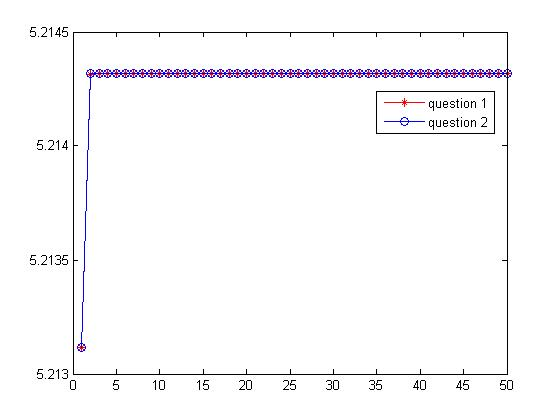
\includegraphics[scale=0.5]{3}

comments:

Both algorithms are very fast to get the right eigenvalues of $A$,
and initial point is also the same, both are 5. But from the graph
of $\lambda_{1}-\lambda_{2}$ below, we can see that algorithm 2 use
less steps to get the final answer, while its computting obviously
comsumes mch more time. 

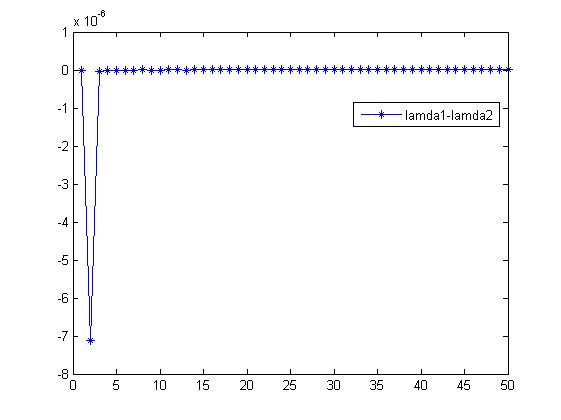
\includegraphics[scale=0.5]{4}
\end{document}
